\begin{frame}
	\frametitle{Content}
	\framesubtitle{ABS-Normal Form}
	\setbeamertemplate{enumerate items}[default]
	\fontsize{12pt}{7.2}\selectfont
	\begin{enumerate}
		\item ABS-NF Einführung
		\item Aufgabengeschreibung
		\item Evaluate
		\item Gradient
		\item Blocksize and Gridsize
		\item Solve
		\item Final Thoughts
	\end{enumerate}
\end{frame}

%------------------------------------------------------------------------
\begin{frame}
	\frametitle{Content}
	\framesubtitle{ABS-Normal Form}
	\begin{columns}[T] % align columns
		\begin{column}{.48\textwidth}
			
			\begin{center}
				{\Huge Einführung ABS-NF}
			\end{center}
			
		\end{column}%
		\hfill%
		\begin{column}{.48\textwidth}
			\color{blue}\rule{\linewidth}{4pt}
			
			\setbeamertemplate{enumerate items}[default]
			\begin{enumerate}
				\item \textbf{Einführung}
				\item Aufgaben
				\item Evaluate
				\item Gradient
				\item Blocksize und Gridsize
				\item Solve
				\item Final Thoughts
			\end{enumerate}
		\end{column}%
	\end{columns}
\end{frame}
%------------------------------------------------------------------------
\begin{frame}
	\frametitle{ABS-NF}
	\framesubtitle{Einführung}
	Ausgangspunkt:
	\begin{itemize}
		\item Picewise smooth functions
		\item Picewise linear function
	\end{itemize}
	\pause
	\begin{figure}[h]
		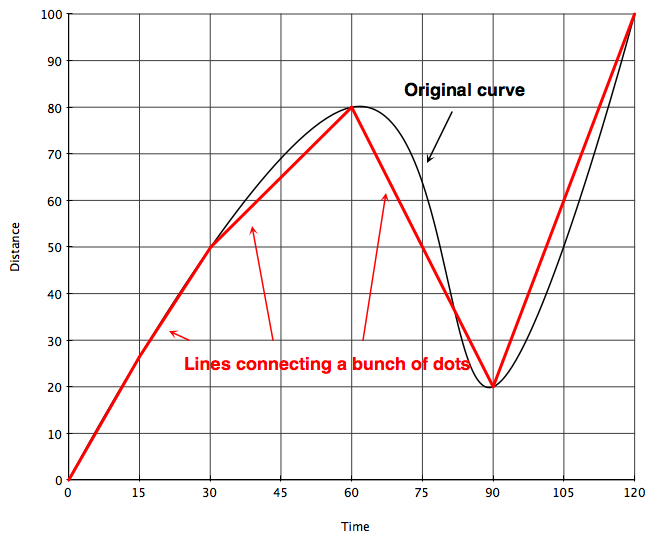
\includegraphics[width=6cm]{img/function}
	\end{figure}
\end{frame}
%------------------------------------------------------------------------
\begin{frame}
	\frametitle{ABS-NF}
	\framesubtitle{Einführung}
	\setbeamertemplate{enumerate items}[default]
	ABS-Normal Form:
	\begin{itemize}
		\item Repräsentierung für Picewise linear functions (PL)
		\item Wird zur Approximierung von picewise smooth functions verwendet
	\end{itemize}
	\begin{flalign*}
	\begin{pmatrix}
	\Delta z \\
	\Delta y
	\end{pmatrix}
	= 
	\begin{pmatrix}
	a \\
	b
	\end{pmatrix}
	+
	\begin{pmatrix}
	Z & L \\
	J & Y 
	\end{pmatrix}
	\times
	\begin{pmatrix}
	\Delta x \\
	|\Delta z |
	\end{pmatrix}
	\end{flalign*}
\end{frame}
%------------------------------------------------------------------------
\begin{frame}
	\frametitle{ABS-NF}
	\framesubtitle{Einführung}
	\setbeamertemplate{ABS-NF}[default]
	Vorgehehen:
	\begin{enumerate}
		\item<1-> (Theorem) Jede PL kann mithilfe von $min$ und $max$ ausgedrückt werden
		\item<2-> (Theorem) Jeder $min$ $max$ Ausdruck kann mit $abs$ repäsentiert werden
		\item<3-> Picewise linearization wird durch algorithmisches differenzieren erreicht.
	\end{enumerate}
	\pause
	
	\begin{center}
		Das Ergebniss ist die ABS-NF einer PL Funktion.
	\end{center}
\end{frame}
%------------------------------------------------------------------------
\begin{frame}
	\frametitle{ABS-NF}
	\framesubtitle{Beispiel}
	\setbeamertemplate{enumerate items}[default]
	\begin{flalign*}
		F(x_1,x_2) &= (x_2^2 - x_1^+)^+ \qquad F : \mathbb{R}^2 \rightarrow \mathbb{R} \\
			 (i)^+ &= \max(0, i)
	\end{flalign*}
	\begin{figure}[h]
		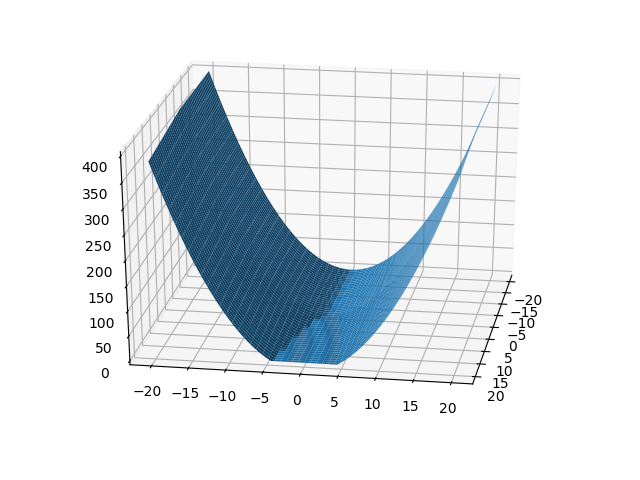
\includegraphics[width=8cm]{img/minmax}
	\end{figure}
	
\end{frame}
%------------------------------------------------------------------------
\begin{frame}
	\frametitle{ABS-NF}
	\framesubtitle{Beispiel}
	\setbeamertemplate{enumerate items}[default]

Nach der Transformation:
\begin{flalign*}
\begin{pmatrix}
\Delta Z_1 \\
\Delta Z_2 \\
\hline
\Delta Y
\end{pmatrix}
&= 
\begin{pmatrix}
w_1 \\
w_7 - \frac{1}{2} |w_1| \\
\hline
\frac{1}{4} |w_1| - \frac{1}{2} |w_7|
\end{pmatrix} +
\begin{pmatrix}
1 & 0  & 0 & 0 \\
\frac{1}{2} & 0 & \frac{1}{2} & 0 \\
\hline 
- \frac{1}{4} & w_2 & - \frac{1}{4} & \frac{1}{2}
\end{pmatrix}
\times
\begin{pmatrix}
\Delta x_1 \\
\Delta x_2 \\
\hline
|\Delta Z_1 | \\
|\Delta Z_2 |
\end{pmatrix}
\end{flalign*}
\begin{flalign*}
	\begin{pmatrix}
	\Delta z \\
	\Delta y
	\end{pmatrix}
	= 
	\begin{pmatrix}
	a \\
	b
	\end{pmatrix}
	+
	\begin{pmatrix}
	Z & L \\
	J & Y 
	\end{pmatrix}
	\times
	\begin{pmatrix}
	\Delta x \\
	|\Delta z |
	\end{pmatrix}
\end{flalign*}
\end{frame}